\section{Insertion Sort} \label{cap:2:section:isort}

\subsection{Introdução}

O Insertion Sort é um algoritmo de ordenação relativamente eficiente com número de entradas baixo,
seu funcionamento consiste em consumir o vetor a ser ordenado de forma sequencial buscando pela
localização correta para o elemento no vetor e inserindo-o na mesma.

\subsection{Implementação}

Para o algoritmo de ordenação baseado em inserção, o pseudo-código utilizado para desenvolver o
algoritmo pode ser observado em \ref{insertionSortP}.

\begin{pseudocode}[caption={Algoritmo de ordenação por inserção}, label={insertionSortP}]
INSERTION-SORT(A)
n $\gets$ len(A)
i $\gets$ 2
while i < n do
    j $\gets$ i
    while j > 1 and A[j - 1] > A[j]
        swap(A[j - 1], A[j])
        j $\gets$ j - 1
    i $\gets$ i + 1
\end{pseudocode}

Esse pseudo-código foi implementado na linguagem de programação C 
e pode ser observado no código seguinte:

\begin{lstlisting}[style=CStyle]
void iSort(int * v, int n)
{
    int j, i;
    i = 1;
    while(i < n)
    {
        j = i;
        while(j > 0 && v[j - 1] > v[j])
        {
            swap(&v[j - 1], &v[j]);
            j -= 1;
        }
        i += 1;
    }
}
\end{lstlisting}
    

\subsection{Análise do algoritmo e notação assintótica}

Para que seja determinada a razão de crescimento do algoritmo de ordenação por inserção, é necessário
perceber os tempos de execução de cada linha do pseudo-código \ref{insertionSortP}.
Nesse caso, pode-se ter como base a equação \ref{cap:2:eq:insertionSort:1}.

\begin{equation} \label{cap:2:eq:insertionSort:1}
    T(n) = C_2 + C_3 + \sum_{i=1}^{n}(C_4 + C_5 + C_9) + \sum_{j=1}^{n^2}(C_6 + C_7 + C_8) 
\end{equation}

Portanto, é plausível relacionar \ref{cap:2:eq:insertionSort:1} com \ref{cap:2:eq:insertionSort:2}.

\begin{equation} \label{cap:2:eq:insertionSort:2}
    T(n) = an^2 + bn + c \  para\  a = (C_6 + C_7 + C_8),\  b = (C_4 + C_5 + C_9)\  e\  c = (C_2 + C_3)
\end{equation}

Com isso, pode-se determinar as seguintes notações assintóticas para o algoritmo de ordenação 
por inserção:

\begin{align*} \label{cap:2:eq:insertionSort:3}
    O(n) &= n^x \forall x \geq 2 \\ 
    \Omega(n) &= n^x \forall x \leq 2 \\
    \Theta(n) &= n^2
\end{align*}

\subsection{Comparação teórica-prática}

Para melhor compreensão do tempo de execução do algoritmo de ordenação por inserção, pode-se observar o gráfico
em \ref{cap:2:graph:insertionSort} que apresentam o tempo de execução para o algoritmo de ordenação por inserção
para 2048 casos diferentes com o número de entradas $n$ variando de 1 a 65536.

\begin{figure}[h]
    \centering
    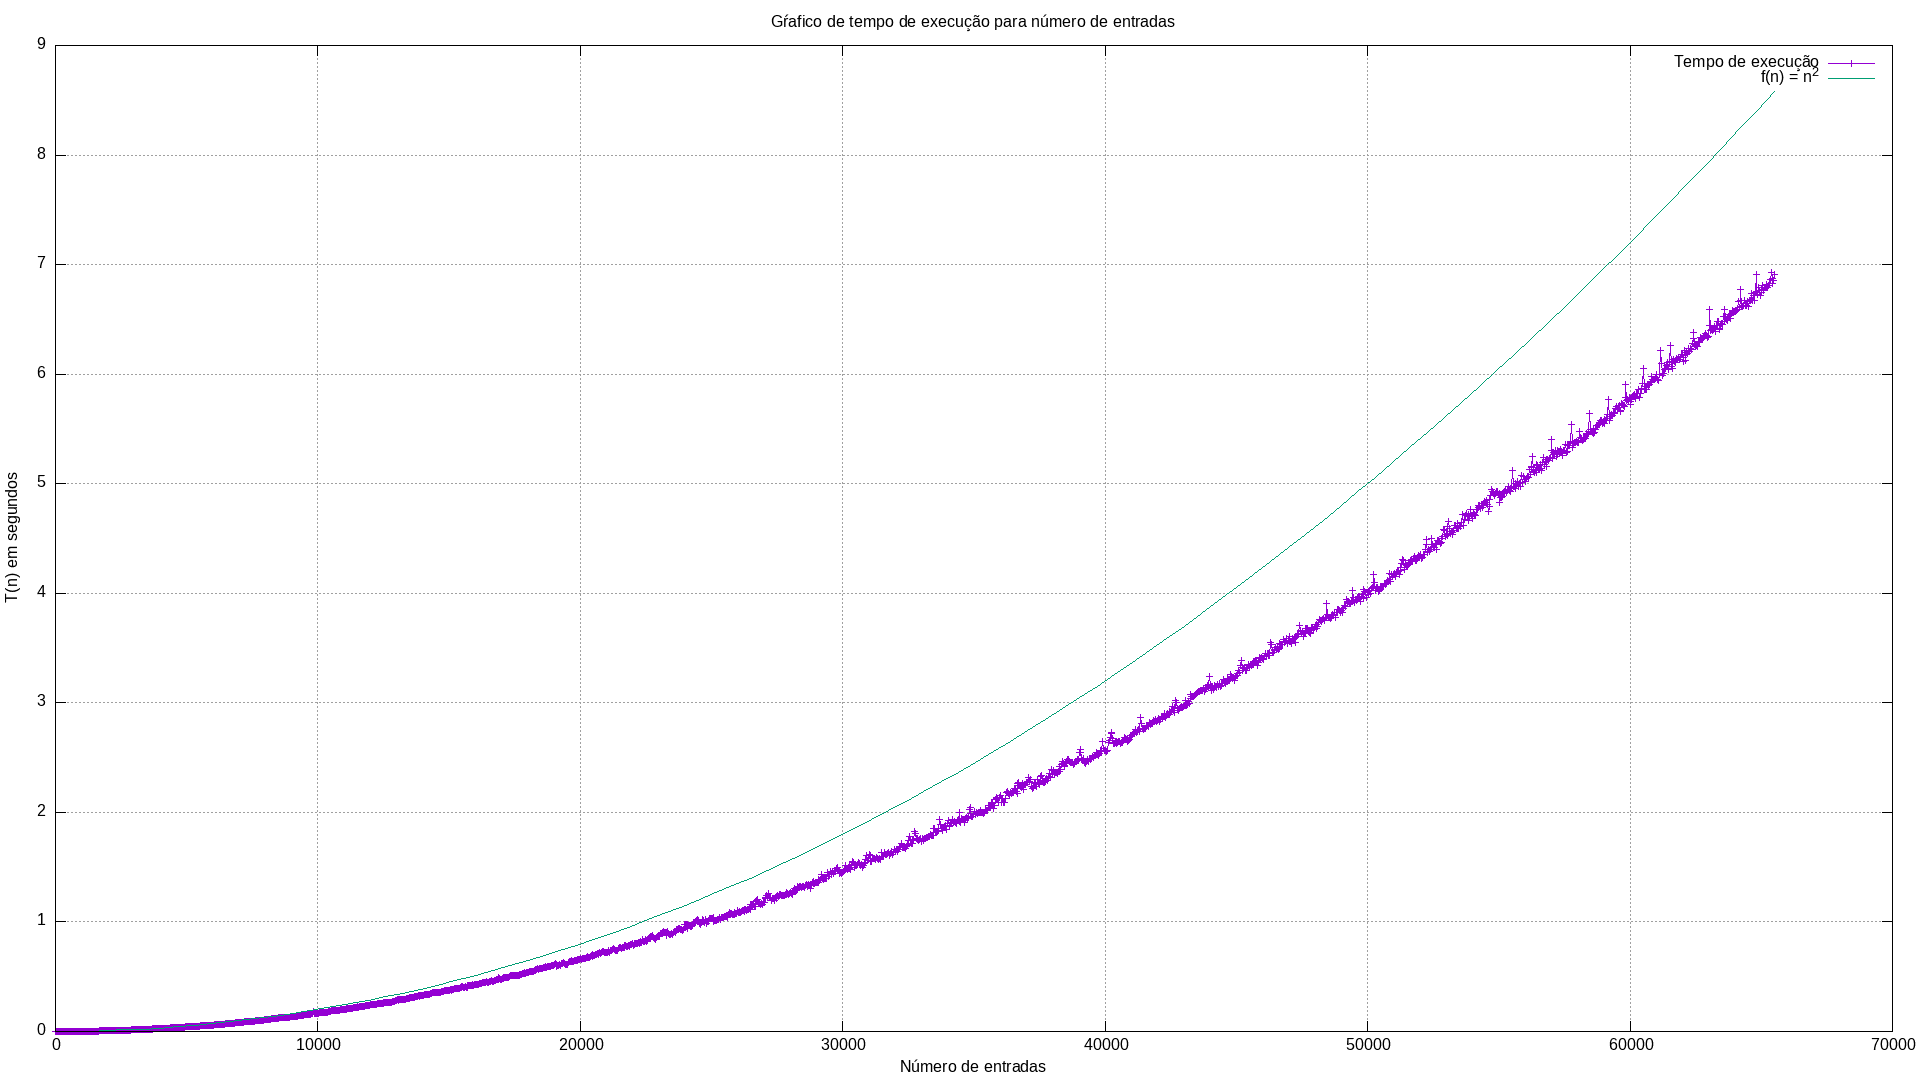
\includegraphics[width=\textwidth]{image/graphics/insertionSort.png}
    \caption{Gráfico com tempo de execução do algoritmo de ordenação por inserção}
    \label{cap:2:graph:insertionSort}
\end{figure}

No gráfico \ref{cap:2:graph:insertionSort}, é possível perceber que o tempo de execução do algoritmo se aproxima
da função $f(n)$ que é uma função quadrática para $n$ com uma redução de escala para melhor percepção e comparação. Então,
utilizando como base o gráfico \ref{cap:2:graph:insertionSort}, pode-se confirmar que a ordem de crescimento determinada é
precisa.

\subsection{Discussão sobre tempo de execução e uso de memória}

Sobre seu tempo de execução, o algoritmo de ordenação por inserção é eficiente para vetores
com poucas entradas a partir de um certo limiar e do contexto, existem outros algoritmos de ordenação
mais eficientes que o mesmo. Sobre seu uso de memória, é constante porque utiliza apenas algumas variáveis
auxiliares.

